\chapter{Introduction}\label{chap:intro}


Wireless sensor networks (WSNs) have recently emerged as a promising computing platform for many nontraditional applications, such as wildfire monitoring in the forest, wildlife tracing in the deep ocean, and intelligence surveillance in the battle field. A WSN usually consists of hundreds of sensor nodes that are equipped with the sensors to measure the physical phenomena, such as temperature, humidity, pressure, or movement of objects. Sensing results are constructed into data packets and routed back to sink nodes, which are typically more powerful, user accessible and have fewer energy constrains.

\begin{figure}[h]
\centering
\mbox{\subfigure[Mica2 sensor]{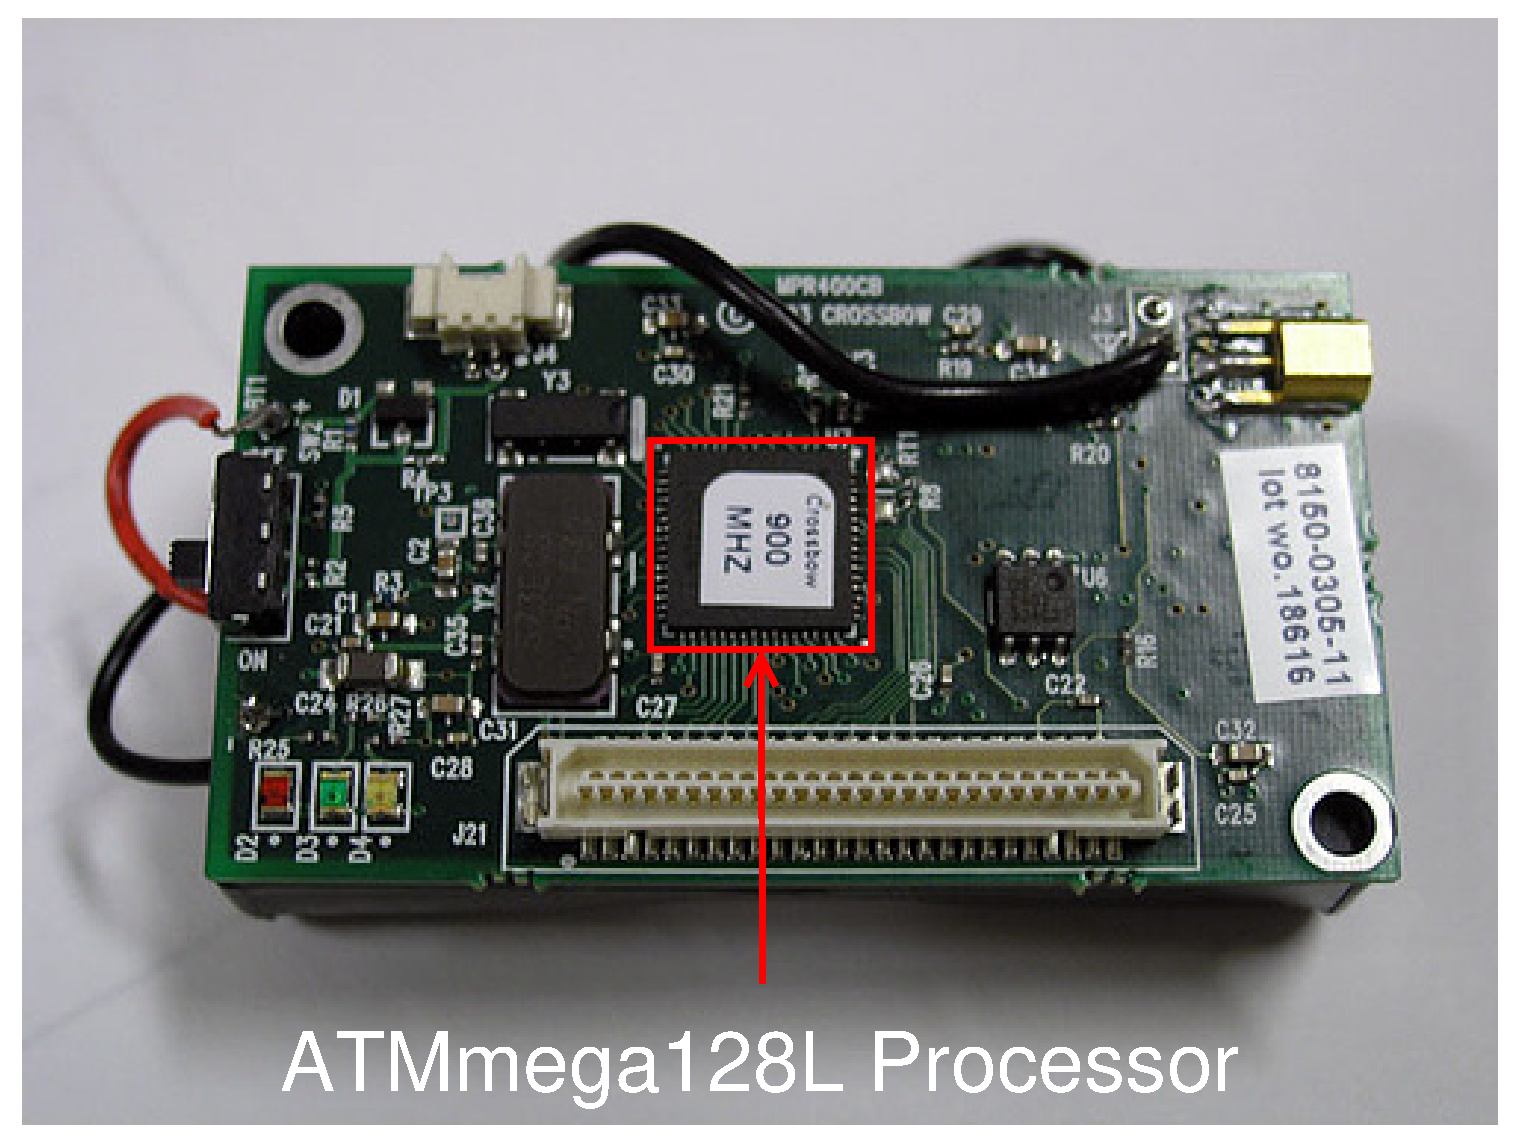
\includegraphics[width=2.6in]{figures/mica2.eps}}
\subfigure[Mica2 block diagram]{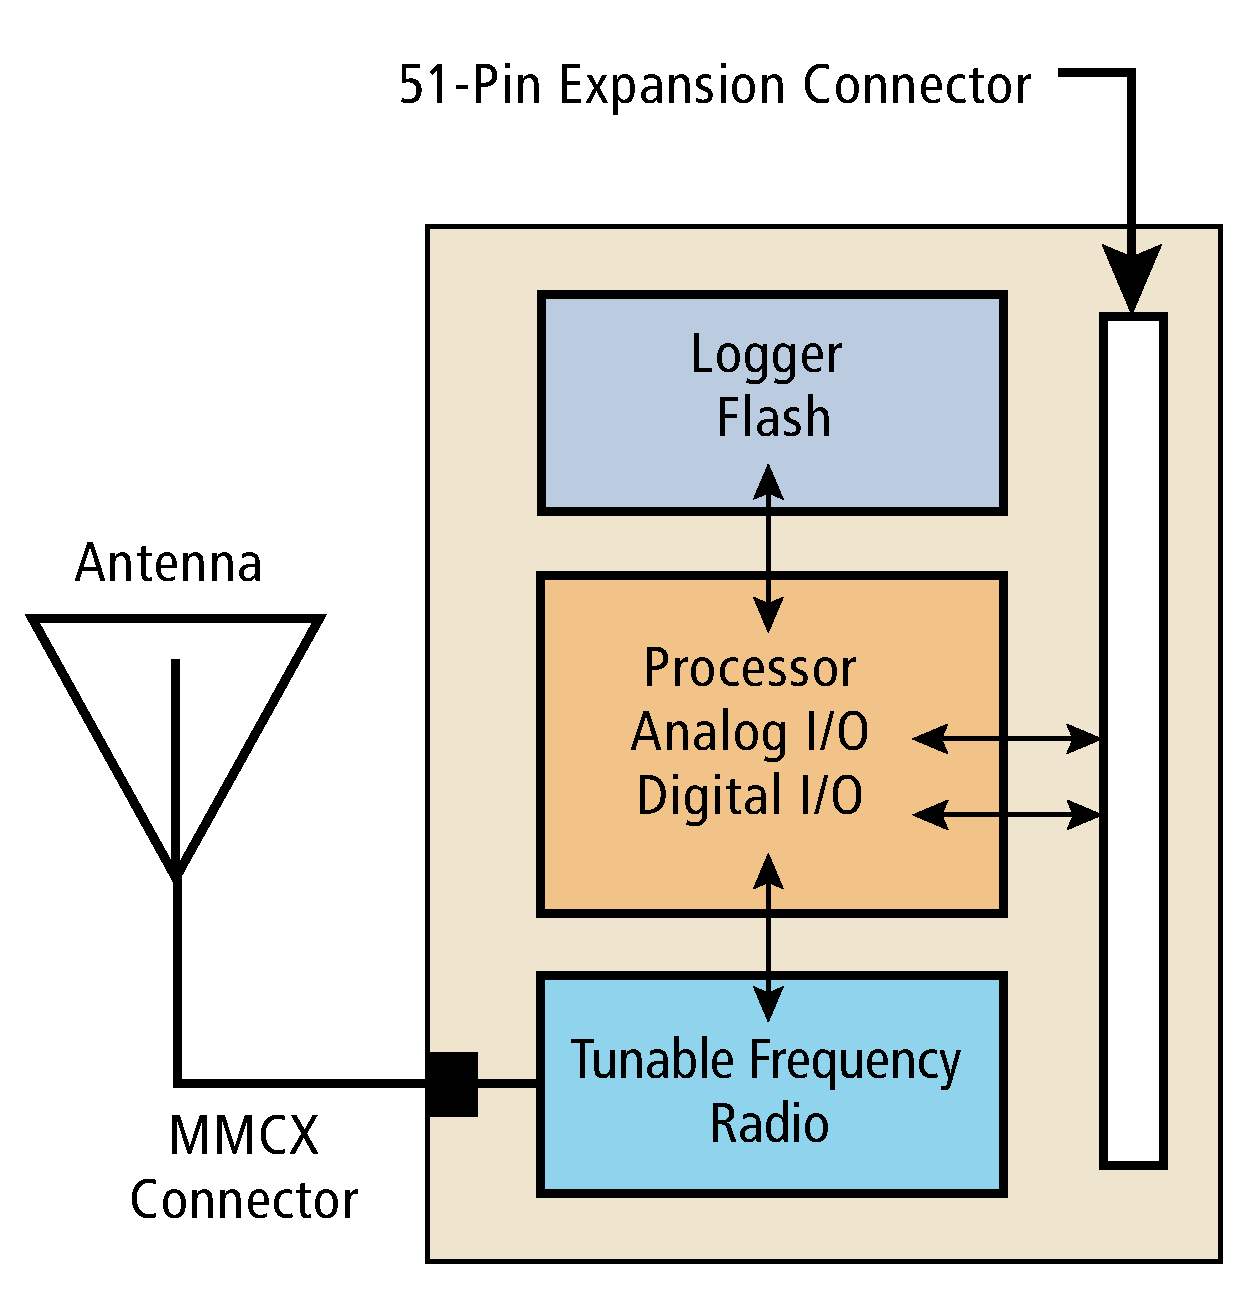
\includegraphics[width=2.8in]{figures/mpr400.eps}}}
\caption{Mica2 sensor and the block diagram.}
\label{fig:mica2}
\end{figure}

The sensor nodes are mainly equipped with processors, sensing devices and communication transceivers. Because they get limited power supplies from the batteries, the simple sensor nodes~\cite{mica2-power, micaz-power,telos,telosb} are equipped with single low power consumption processor. 
For example, a Mica2~\cite{mica2-power} mote shown in Figure~\ref{fig:mica2}, is equipped with a 8MHz ATmega128L processor to process the sensed data.

With the technology advances, sensors equipped with multiple chips~\cite{imote2} have been proposed recently. Shown in Figure~\ref{fig:imote2}, Imote2~\cite{imote2} developed by Intel has a DSP chip on the mote, besides the CPU core, to support image and video operations. The multi-chip sensor is now able to pre-process the multimedia content sensed by the equipped camera and microphone, so that the package that needs to be sent back to the sink contains only a summary of the sensed results.

\begin{figure}[h]
\centering
\mbox{\subfigure[Imote2 sensor]{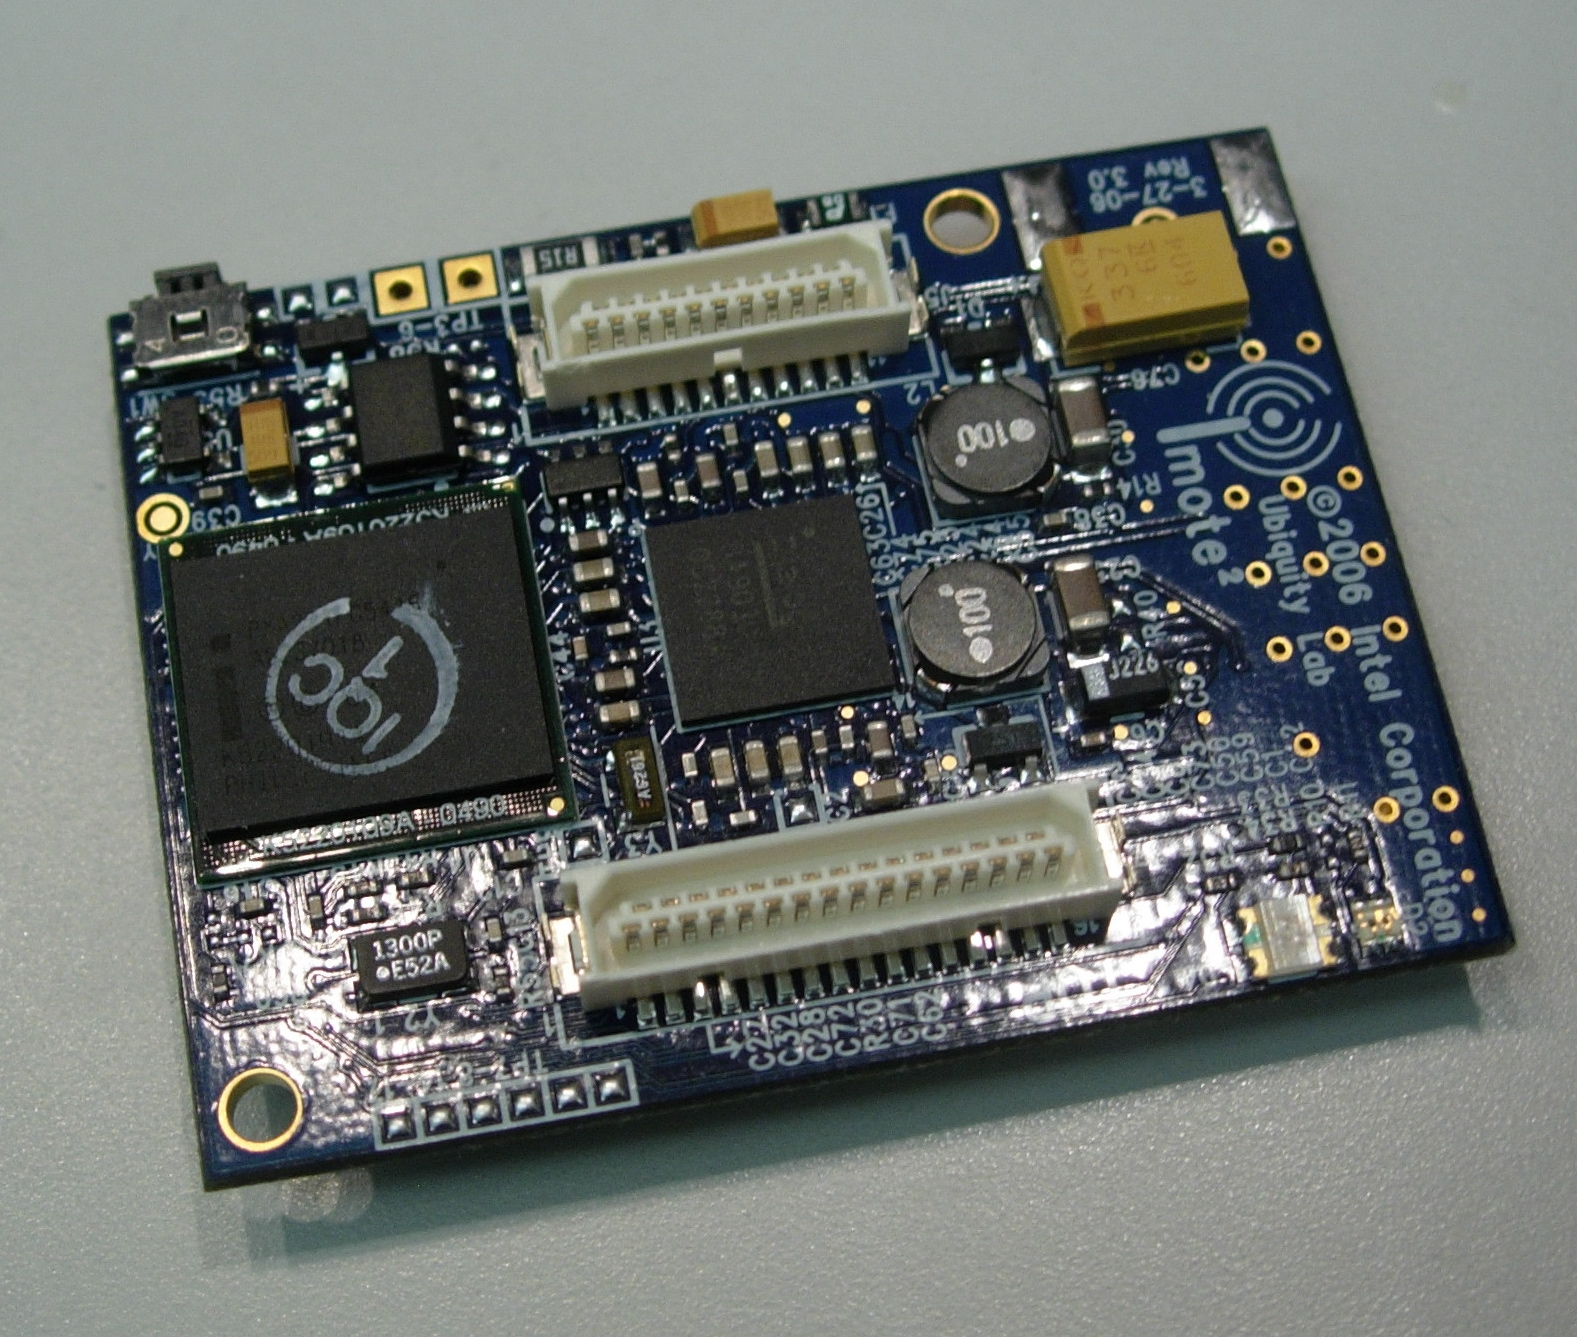
\includegraphics[width=1.8in]{figures/imote2.eps}}
	\hspace{20mm}
      \subfigure[Imote2 block diagram]{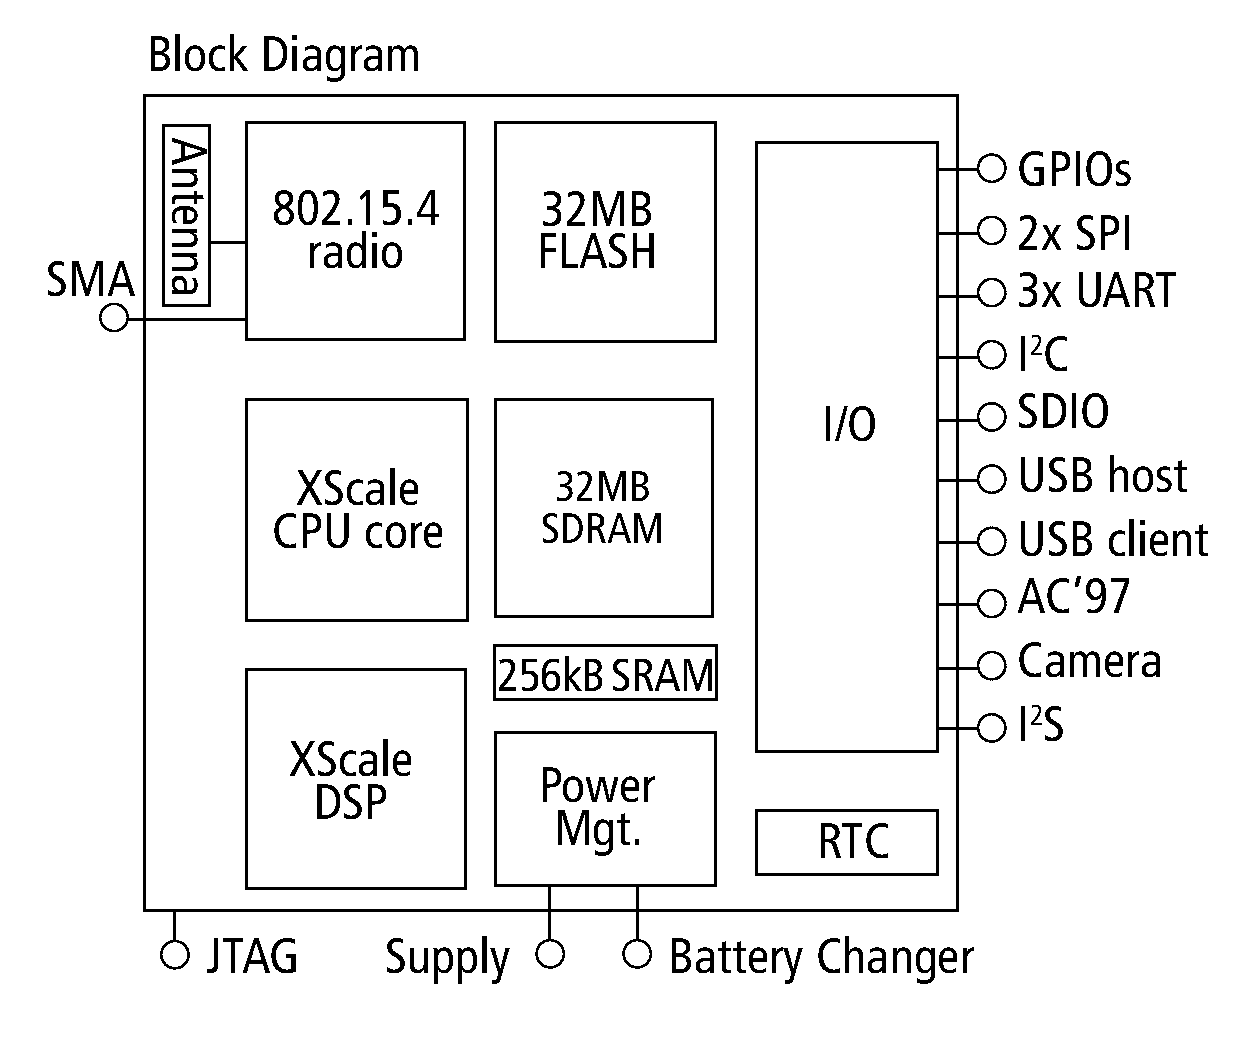
\includegraphics[width=2.8in]{figures/imotedia.eps}}}
\caption{Imote2 sensor and the block diagram.}
\label{fig:imote2}
\end{figure}

The availability of multi-chip sensors  brings a lot of design opportunities into WSN study. The high manufacture cost of these sensor nodes makes it economically less appealing to let the whole network run just one application. Recently, researchers have envisioned the wide adoption of multi-application wireless sensor networks (MA-WSNs), which can support application concurrency in one network infrastructure~\cite{melete,ma-wsns}. Besides that, MA-WSNs are also able to execute different applications interleavely on one sensor node.


Compared to single-application wireless sensor networks (SA-WSNs), MA-WSNs have many advantages, in terms of efficiency and flexibility.
For example, MA-WSN can be deployed in a national park to monitor both wildfires and animal movement. More sensors can be set to monitor the animal movements in the early morning or late afternoon when animals tend to hibernate; and more sensors could be set to monitor wildfires in summers when there is a higher probability to catch a fire. By exploiting the same network infrastructure for both events, (1) MA-WSNs save the investment and effort of deploying and testing two sensor networks; (2) the sensor network adapts better to the dynamic changing environment and even adjusts the coverage according to the need.

\textbf{Software upgrade.}
In both SA-WSNs and MA-WSNs, the applications running on the sensors may need to be upgraded after the deployment.
Bug fix or feature enhancement are the common reasons for software upgrade.
Especially, when the application is still under development, testing and debugging may take several rounds until the code is stable.
For example, the WSN may be deployed in an area which human beings are not familiar with. After the sensor nodes are deployed, data will be collected and sent back to the sink node. With more knowledge about the environment, the scientists may be able to adjust the sensing functions to make them more accurate based on the preliminary data analysis. I formulate updating code or data of a running application in the network as the software upgrade problem in WSN software update. As shown in Figure~\ref{fig:upgrade}, software upgrade involves binary code generation on the sink node, patch deployment and image replacement on the sensor nodes.
\begin{figure}[htbp]
	\centering
		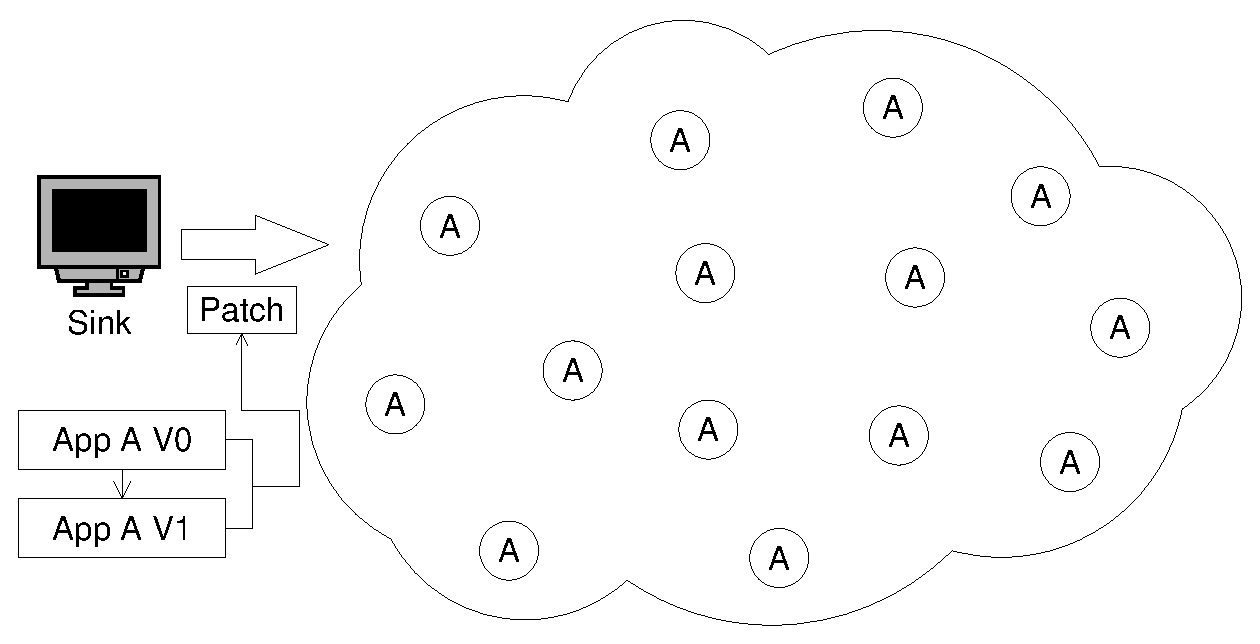
\includegraphics[scale=0.45]{figures/upgrade.eps}
	\caption{Software upgrade in a WSN.}
	\label{fig:upgrade}
\end{figure}
Because the sensors are usually left unattended after deployment, the patch deployment can only be done via wireless communication.
 This is an expensive operation in WSNs. For large WSNs, where the code source cannot reach destinations via broadcasting, the package has to be transmitted hop-by-hop in the network, which consumes a significant amount of energy. Recent study~\cite{related:barr-energy} has shown that it consumes about the same amount of energy as executing 1000 instructions to send a single bit of data one hop away in WSN. As the sensor nodes are running with limited power supplies, it is essential to conserve the energy in a WSN during software update, especially when it happens frequently.
 
One possible solution to this problem is to reduce the number of bytes that need to be transmitted during software upgrade. Because the update patch is actually the binary level difference between the old and new code image, minimizing the binary level difference while generating the new binary will reduce the patch size, thus reduce the energy consumed by transmitting the patch in the WSN. A wise design of how to format the patches may also help to reduce the patch size.
A good patch distribution protocol can also reduce the energy consumed in the software upgrade procedure.


\textbf{Software switch.}
For SA-WSNs, software upgrade is the major reason to update the binary image on the sensors, but for WA-WSNs, there is another code update circumstance that can happen.
In order to support application concurrency, multiple code images can be preloaded to the sensor nodes before deployment, and the sensors are able to switch between them upon request from the sink node. However, because of the memory size limitation, not all the code images can be stored on the sensors. This will require the sensors to fetch the binary of the wanted yet unavailable application from somewhere else. The source can be the sink node, or the neighboring sensors that own this code image. Shown in Figure~\ref{fig:switch}, while doing software switch, only a subset of the sensors in the network need to download the application.
This is different from the software upgrade, where all the sensors need to download the new image. Also, both the sink node and the other local sensors may act as code sources, while in software upgrade, only the sink node can be the source.
\begin{figure}[htbp]
	\centering
		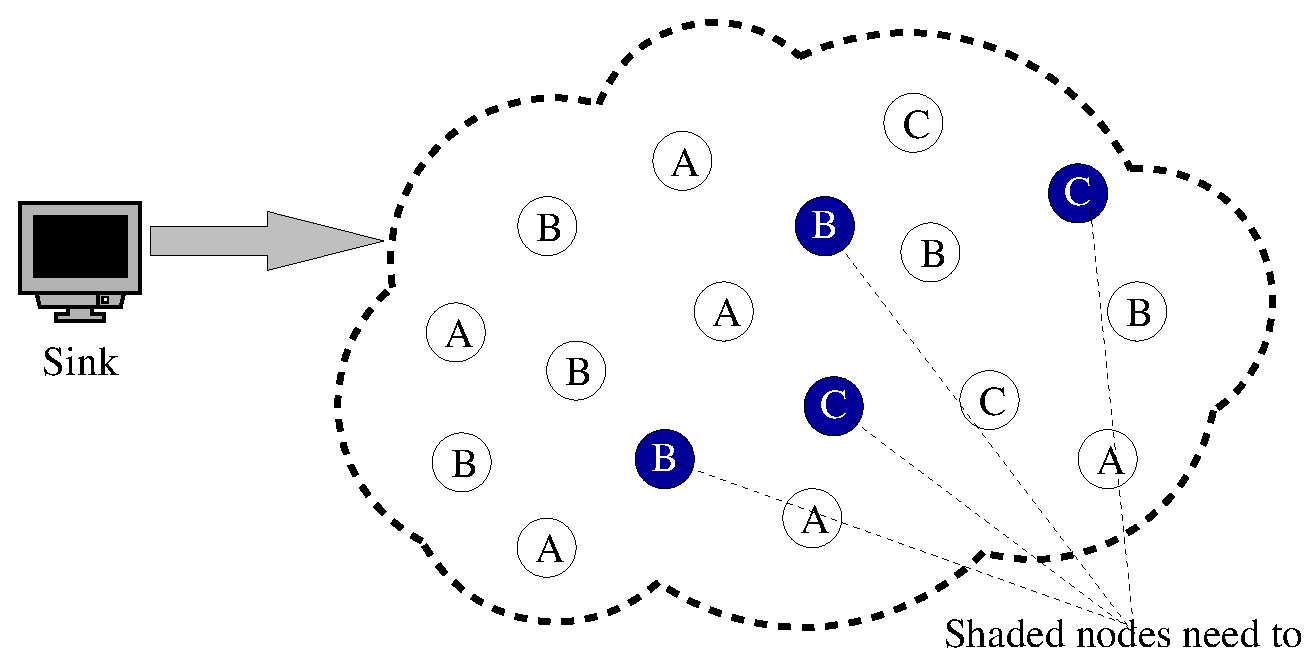
\includegraphics[scale=0.45]{figures/switch.eps}
	\caption{Software switch in a WSN.}
	\label{fig:switch}
\end{figure}

Similar as the software upgrade problem, in order to reduce the energy consumption during the software switch, an energy-efficient patch routing design and a good patch format design are both desired. 
As different sensor applications may share same components, there are usually identical parts between the binaries of those applications. For example, in the sensor operating system TinyOS~\cite{tinyos}, there is a component called ``Leds'' that manages the colors, on and off of the led lights installed on the sensors, and it is commonly used in many sensor applications such as ``Blink'' and ``CntToLeds''. 
One possible solution here is to generate the same binary for the shared part and using differential patching to transmit only the binary difference between the two applications instead of the whole new image should reduce the number of bytes that need to be transmitted during software switch.

Based on the above discussion, we can see that both software upgrade and software switch can happen frequently in WSNs. The patch transmission highly relies on wireless communication, therefore, it is a costly execution in WSNs.
One of the great benefits that WSNs bring is the spontaneity. Once the WSN is set up, it can sense and report
the environmental information automatically.
However, the high power consumption in the software update procedure will affect the lifetime of the WSN.
As the sensors are usually hard to access after deployment, it will require a lot of human resource or even impossible to replace the batteries. New sensors may be purchased to replace the old ones, but this is neither economical nor environmental friendly.

\section{Overview of this research}

No matter whether the software update is caused by software upgrade or software switch, in summary, there are three steps in the software update procedure.
The compiler generates the binary image(s).
The patch generator produces the patch.
Then, the patch is disseminated to the WSN. After the sensor gets the complete patch, it will rebuild the target binary , load it to program memory and start running it.

In order to solve the software update problem in WSNs under all the resource constraints, this dissertation presents a software update management framework, as shown in Figure~\ref{fig:overview}. 
The sink node represents a computer server, that is not resource constrained hypothetically. The sensor network consists of a large number of sensor nodes with resource limitations, in terms of energy, memory size,  network bandwidth, time, and CPU computation ability.

\begin{figure}[htbp]
	\centering
		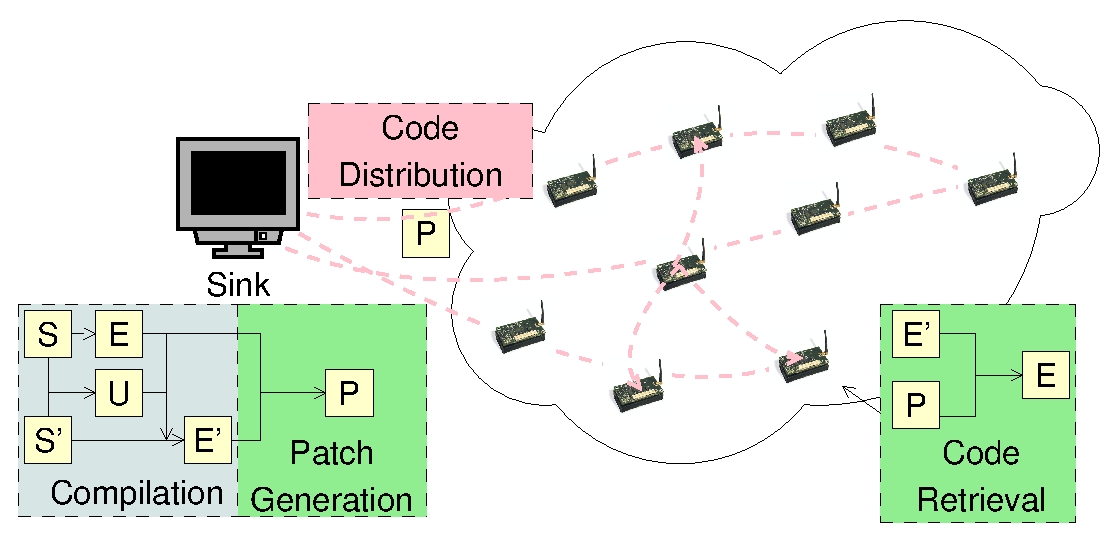
\includegraphics[scale=0.45]{figures/model.eps}
	\caption{Software update framework overview.}
	\label{fig:overview}
\end{figure}


The compiler first compiles the source code into executable binary {\it E'}. 
Instead of sending the new binary image, a small sized patch {\it P'} is distributed over the network, which only contains the differences between the new binary {\it E'} and the binary base {\it E}.  After code distribution is complete, the target sensor regenerates the new binary code {\it E'} by combining the received patch {\it P} and the preloaded binary base {\it E}. 

This framework includes three major components.

\textbf{Update-conscious compiler.} 
Because the patch transmitted over the network is the binary level difference between the old binary and the new  binary, increasing the binary level similarity between the two versions can reduce the number of bytes that need to be transmitted. Therefore, it will save both energy consumption and transmission time in software update. 


In the new version of source code, the source level statements can be divided into two categories, the changed and the unchanged statements.  The modified source statements will produce binary level differences, and these binary changes are difficult to avoid, yet the source level statements that are not changed may also create binary differences.
This is because in the code generation phase, the compiler is able to produce different binary statements that have the same semantic meanings, according to the contexts.

In this dissertation, I will propose the UCC techniques, that reads the old source and binary to get the compilation choices of the old version, and use them as hints while generating the new binary. 
Shown in Figure~\ref{fig:overview}, UCC takes {\it E} (the old binary), {\it U} (the intermediate level differences between the old version and the new version), and {\it S} (the new source code) as inputs, to generate the new binary {\it E'}. A similar compilation option is chosen while generating the new binary, thus, this technique can improve the code similarity between the old and new binaries.

This dissertation focuses on the UCC register allocation and data allocation schemes for general purpose and DSP applications.
It proposes the ILP based UCC register allocation (UCC-RA) and the heuristic based UCC data allocation (UCC-DA) for general purpose compilation.
The incremental coalescing single/general offset assignment algorithms are designed for the DSP compilation as the UCC data allocation and UCC address register allocation schemes.

The goal of UCC is to minimize the binary level differences, it may not generate the most efficient code as the conventional compilers does.
In fact, it trades the run-time code performance for binary similarity, in other words, it saves energy in software update but wastes the run-time energy.
If we consider the software update and the execution before the next update as a whole procedure, UCC may not save the energy for the whole procedure and prolong the WSN's life time.
In order to solve this problem, I studied the trade-off between the binary code differences and run-time performance. An adjustable UCC scheme is presented in order to achieve the best balance, thus the energy saving for the whole procedure.
	
\textbf{Patch generator.}
After the new binary {\it E'} is generated, it is then compared with the old binary {\it E} to generate the update patch. The binary level differences are described in a highly condensed script {\it P}. 
From the preliminary experimental results, I found that multiple binary level differences can result from the same cause, e.g., instruction insertion or removal can cause destination address shift for the branch instructions.
Including the common cause instead of the individual changes should be able to reduce the patch size.
However, if the update script design is too complicated, it will require more effort on the sensor side to decode and regenerate the target new binary.
This dissertation presents several sets of the script primitives, and the trade-off between the patch transmission effort and the sensor side decoding effort.


\textbf{Code distribution protocol.}
The code distribution protocol disseminates the patch packets to the destination sensors that need such software update. The code source can be the sink node or the other sensors that own the requested binary image.
This dissertation presents 
a code distribution scheme that works for both software upgrade and software switch circumstances.

The presented network protocol also runs under the WSN constraints.
The wireless links in WSNs are not stable. Both the communications and nodes are unreliable, because of the environment where the WSN is deployed and the limited energy resources of the sensors. The network protocol has to be robust enough to tolerate link failure and node failure in the WSN.
Because of the high bandwidth and memory usage, the sensors may not be able to perform the sensing applications during the software update procedure. In order to reduce the down time of the sensors, the software update procedure is desired to be as fast as possible. 
Thus, the code distribution protocol design should disseminate the patch scripts to the WSN with the less amount of traffic and time.

%\section{Challenges}
%
%In this research, I focus on the WSNs, that are built with low-power sensors such as the Mica2 sensors~\cite{mica2-power}. They consist of a 8 MHz ATmega128L processor, 128KB of program memory, 512KB EEPROM, 4KB of data memory, and a multi-channel radio capable of transmitting at 38.4 Kbps with an outdoor transmission range of approximately 500 feet. The device measures 2.25 inch $\times$ 1.25 inch $\times$ 0.25 inch and is typically powered by two AA batteries.
%
%The major constraints of designing an energy-efficient software update management framework for such kind of sensor networks are addressed as below.
%
%\textbf{Energy constraints.}
%The environment usually makes it hard to physically access the sensors after deployment, so it is difficult to replace the batteries for the sensors. Recharging the batteries using natural energy sources is not trivial, because the network might be set up in the area, such as the deep ocean, where it is hard to get access of sun light or other natural energy sources. 
%
%Take the Mica2 sensor as an example. The energy contained in each AA battery is 15,390 Joule~\cite{battery-energy}. The experiment results in the recent study~\cite{power-tossim} showed that the energy consumption of the selected applications running on the sensors varies from 153.7 to 3,689 J/day, which makes the life time of the sensors to be 8 days to 200 days. Thus, developing an energy-efficient software update method is very important for energy limited WSNs.
%
%
%\textbf{Memory constraints.}
%The active program is stored in the program memory of a sensor node, while the other inactive programs are stored in the external flash memory. Sensor nodes will load the code image from the external flash to the program memory when they need to switch the running application from one to another.
%
%However, due to the limited size of the external flash memory, the sensor node may not be able to store the complete code images of all the applications that it needs to run. This requires the sensor node to download the unavailable code image from the sink node or the other neighboring nodes during software switch. How to design an energy-efficient code fetching scheme is a problem that we need to solve.
%
%Although the sensors can fetch the wanted code image upon request, the limited sensor memory still needs to be divided wisely to store multiple code images. When the memory is not big enough to hold all the code images, an eviction scheme will be needed.
%
%
%\textbf{Computation constraints.}
%A sensor node is typically equipped with MHz (instead of GHz) micro-controller(s), which limits the complexity of  applications running on it. Therefore, the software update application that runs on the sensors has to be lightweight.



\section{Assumptions}
The following assumptions are made to simplify the implementation of the software update framework in WSNs.

\textbf{Multiple software update procedures on one sensor do not interleave with each other.}
Although it is possible that multiple applications can co-exist on one sensor node, there is a small chance that the software update to these applications happen at the same time.
Also, because the sensors can only run one application at a time, it is not necessary to update them at the same time.
Update sequence can be determined by the order of release time or the execution frequencies.

\textbf{The binary is transmitted during software update.}
A typical compiler like GCC can take over 100K memory space, therefore, it is not practical to install compilers on the sensors.
Therefore, we cannot send the source code to the sensors and let them compile the new binary.
Some designs let the sensors run virtual machine instructions or high level instructions instead of the binary instructions in order to reduce the code size~\cite{mate,related:dynamic1, related:dynamic2}. However, these methods introduce some run-time overhead, which may not be acceptable for tightly resource-constrained embedded system, so optimizing the software update procedure for the virtual machine design is not discussed in this research. However, it can a future research opportunity.

\textbf{The mapping between the source code and the binary can be built.} Compiler optimizer may re-order the instructions in order to achieve better run-time performance. Therefore, the update-conscious compilation techniques should execute as a separated pass after the other compiler optimizations. 
We assume that the compiler can create the mappings between the optimized binary statements and the source statements to categorize the binary level differences into the functional changes and nonfunctional changes.
The update-conscious compiler will then decrease amount of the nonfunctional binary changes.
Mappings between the unoptimized and optimized statements can be created by using the technology proposed by~\cite{mapping}.


\textbf{The number of execution of one application can be estimated.}
As the software engineers who design the application should be able to estimate how often one execution can be trigged, and the lifetime of one application can be estimated by the historical release logs, the number of execution that one application will do before retiring can be estimated. This number acts as a constant for each application in the energy consumption formula and determines the compilation strategy that will be used to generate binary in the adjustable UCC algorithms.

\section{Organization of this dissertation}
The remainder of this dissertation is organized as follows. 
Chapter 2 presents background information on the general WSN software update and the three components of 
the proposed framework, including traditional register allocation,
data allocation design, WSN software update script primitive design and WSN code dissemination protocol design.
Also, the relationship of this dissertation and prior work is discussed. 
Chapter 3 discusses the proposed UCC design, including the UCC register allocation and data allocation for
general purpose applications and the UCC data allocation and address register allocation for DSP applications.
Chapter 4 presents the script primitives that are used to summarize the binary level differences
in the update patch.
In Chapter 5, the patch distribution protocol is presented. 
Chapter 6 presents the experimental results and discusses the trade-offs.
Chapter 7 addresses the directions for future
research and the conclusion.
